{n个结点的二叉链表中含有n+1个空指针域。利用二叉链表中的空指针域,存放指向结点在某种遍历次序下的前趋和后继结点的指针(这种附加的指针称为``线索'')。{这种加上了线索的二叉链表称为线索链表,相应的二叉树称为线索二叉树。}线索二叉树的结点结构定义如下:\\
}

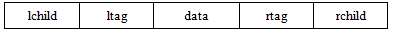
\includegraphics[width=3.70833in,height=0.31250in]{png-jpeg-pics/2C7D92B8C8B6DFA32271B9299B2CFE31.png}

{其中:}

{~ ~ ~ ltag=0时lchild指向左子女;}

{~ ~ ~ ltag=1时lchild指向前驱;}

{~ ~ ~ rtag=0时rchild指向右子女;}

{~ ~ ~ rtag=1时rchild指向后继。}
